%dvipdfmx interim_sample.dvi

\documentclass[a4j, twocolumn]{jsarticle}
\usepackage{dendentitle}
\usepackage{amsmath, amssymb, bm, setspace}
\usepackage{cite}
\usepackage{subfigure}
%\bibliographystyle{junsrt}

\newcommand{\argmax}{\mathop{\rm arg~max}\limits}

\def\vector#1{\mbox{\boldmath $#1$}}
\renewcommand{\figurename}{fig.}
\renewcommand{\refname}{References}

% set margines
\setlength{\topmargin}{-15mm}
\setlength{\textheight}{252mm}
\setlength{\textwidth}{165mm}
\setlength{\oddsidemargin}{0mm}
\setlength{\evensidemargin}{0mm}

\setstretch{1.2}


\usepackage[dvipdfmx]{graphicx}
%\usepackage{apalike}
%\bibliographystyle{apalike}

\title{フェーザ四元数によるPolSAR地表分類\\PolSAR Land Classification Using Phasor Quaternion Neural Networks}
\author{廣瀬研究室 修士過程1年 37-186441 大塚 優太}
\date{2018年11月2日}

\begin{document}

\makedendentitle{輪講資料}{指導教員 廣瀬 明}

\section*{Abstract}
SAR plays a significant role in the remote-sensing earth observation. SAR observations have been conducted globally targetting various areas such as polar regions, tropical areas and the ocean. Polarimetric SAR (PolSAR) is one of the SAR techniques, which uses fully polarized data. With PolSAR, we can obtain the physical information of the scatterers. Hence, PolSAR is a useful technique for land classification. A lot of land-classification methods have been proposed such as entropy methods, decomposition methods and quaternion-neural-networks methods. Conventional methods did not use the data from Interferometric SAR (InSAR) for land classification. We can use both phase and polarization for land classification by using phasor quaternion neural networks(PQNN). In this paper, we tested land classification considering the interferometric phase. The results were better than conventional methods. It means that the interferometric phase can be used to solve the problems in land classification.

\section{はじめに}
合成開口レーダ(Synthetic Aperture Radar : SAR)は、航空機や人工衛星などのように搭載できるアンテナの大きさに制限があるときに空間的に移動しながら観測を行うことで仮想的に大きな開口面のアンテナを作って分解能を高める技術である。

SARは、アンテナ自身から電波を照射し地表面から返ってきた電波を観測する能動型のセンサであるため、夜でも観測を行うことができる。また、波長が長いマイクロ波を用いているので天候に左右されずに観測を行うことができる。これらの利点からSARはリモートセンシングによる地球観測において重要な役割を果たしていて、現在に至るまでSARを使って極地や熱帯地域、海洋などの様々な地域の広域的な観測が継続的に行われている\cite{ouchi}。
 \begin{figure}[!t]
 \centering
 \includegraphics[width=8cm]{alos2.jpg}
 \caption{The SAR satellite(ALOS-2) http://www.eorc.jaxa.jp
}
 \label{fig:SAR}
\end{figure}
複数の偏波を利用する多偏波合成開口レーダ(Polarimetric SAR : PolSAR)の利用先の一つとして地表分類がある。PolSARによって取得された地表からの後方散乱特性の情報を用いると観測した地域を森、草原、湖、街などのカテゴリーに分類することができる。エントロピーによる分類\cite{cloude1997entropy,pottier2000application,lee1999unsupervised}、散乱モデルによる分類\cite{freeman1998three,yamaguchi2005four,singh2018model}、四元数ニューラルネットワーク(Quaternion neural network : QNN)による分類\cite{shang2014quaternion,kinugawa2018isotropization}などが存在する。従来手法では、干渉合成開口レーダ(Interferometric SAR : InSAR)による干渉画像の位相を地表分類に用いることはなかった。干渉画像の位相は地形の高度変化を表しているので地表分類に有効に利用できる。

そこで、本研究ではフェーザ四元数ニューラルネットワーク(Phasor quaternion neural network : PQNN)を使うことによって干渉画像の位相を考慮した地表分類を行う。地表分類では街が森に誤って分類される、水面が波打つことで湖が草原と分類されるなどの問題がある。これらの問題を干渉画像の位相を用いることで解決することを目指す。

\section{干渉合成開口レーダ}
\begin{figure}[!t]
	\begin{center}
		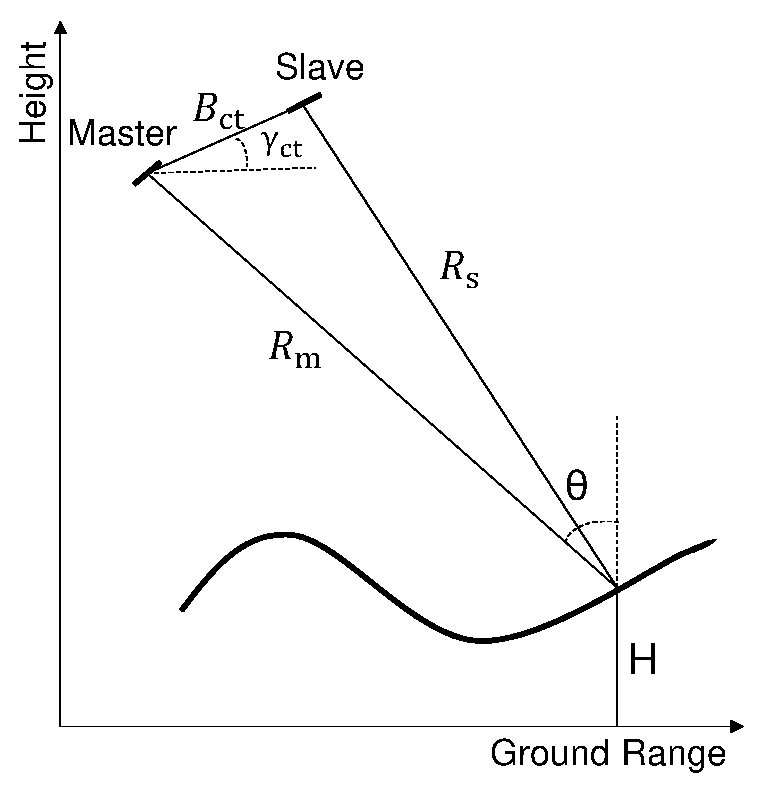
\includegraphics[scale = 0.5,bb=0 0 345 359]{InSAR1.eps}
		\caption{InSARによる観測の様子。}
		\label{InSAR}
	\end{center}
\end{figure}
InSARの原理を以下に示す。
まず、同一地域を二箇所から観測し、masterとslaveと呼ばれる二種類の複素振幅画像を得る。

この二つの複素振幅画像は異なる位置から観測したものなのでずれを補正する必要がある。この作業は位置合わせと呼ばれる。

位置合わせを終えた後、masterとslaveの複素共役積をとることにより干渉画像を得る。この段階では雑音を多く含んでいるので、通常は窓を取って平均した値を1ピクセルの値とするマルチルックという処理を行う。

干渉画像の位相はmasterとslaveの位相差であり、二つのアンテナと地表面との距離の差に対応しているため、幾何的な位置関係から標高を求めることができる。図\ref{InSAR}はアンテナと地表面との位置関係を表している。二つのアンテナと地表面との距離をそれぞれ$R_{\rm{m}}$、$R_{\rm{s}}$、、二つのアンテナの距離を$B_{CT} $、水平面から見た二つのアンテナの角度を$\gamma _{CT} $、地上から見た衛星の仰角を$\theta$、レーダの波長を$\lambda$とする。このとき、干渉画像の位相$\Phi $は以下の式で表される。
\begin{equation}
\frac{\lambda \Phi }{ 2\pi } = 2\left( R_{\rm{m}}-R_{\rm{s}} \right)
\end{equation}
また、幾何的な位置関係から以下の式を得る。
\begin{equation}
\left( R_{\rm{m}}-R_{\rm{s}}\right) = B_{CT} \sin \left( \theta - \gamma _{CT} \right)
\end{equation}
二つの式を連立することにより、$ \theta $と$ \Phi $の関係が求まる。
\begin{equation}
\Phi =\frac{ 4\pi B_{CT} \sin (\theta - \gamma _{CT}) }{ \lambda }
\end{equation}

\begin{equation}
\frac{\Delta \Phi }{\Delta \theta } =\frac{ 4\pi B_{CT} \cos (\theta - \gamma _{CT})}{\lambda }
\end{equation}
また、標高$H$と$\theta$には以下の関係がある。
\begin{equation}
\frac{\Delta H}{\Delta \theta } =R_{\rm{m}} \sin (\theta )
\end{equation}
(4)、(5)を連立することで、標高と位相の関係を求めることができる。
\begin{equation}
\frac{\Delta H}{\Delta \Phi } =\cfrac{\lambda R_{\rm{m}} \sin (\theta )}{ 4\pi B_{CT} \cos (\theta - \gamma _{CT})}
\end{equation}
\begin{equation}
\Delta H=\frac{\lambda R_{\rm{m}} \sin (\theta )}{ 4\pi B_{CT} \cos (\theta - \gamma _{CT})}\Delta \Phi
\label{dhdp}
\end{equation}
以上の式より、干渉画像の隣接ピクセルの位相差を足していくと標高を計算できることがわかる。

\section{フェーザ四元数ニューラルネットワークによる地表分類}
\subsection{フェーザ四元数}
大山ら\cite{oyama2018phasor}によって提案されたフェーザ四元数は四元数部分と単位フェーザ部分から構成され、次式のように表される。
\begin{eqnarray}
	{\bf x} &\equiv& {\bf x}^{q}{\bf x}^{p} \nonumber \\
	&\equiv& \left[\begin{array}{ccc}x^{r}\\x^{i}\\x^{j}\\x^{k}\end{array}\right]\exp(i\phi)
\end{eqnarray}
${\bf x}^{q}$が四元数部分であり、一つの実数$x^{r}$と三つの直交する虚数$x^{i}$,$x^{j}$,$x^{k}$から成る。${\bf x}^{p}$は単位フェーザ部分であり、振幅を1、位相を$\phi$とした複素数である。

フェーザ四元数の和は以下のように定義される。
\begin{eqnarray}
	{\bf x}_{1} + {\bf x}_{2} &\equiv& ({\bf x}^{q}_{1} + {\bf x}^{q}_{2})\exp(i\phi) \nonumber \\
	&=& \left[\begin{array}{ccc}x^{r}_{1} + x^{r}_{2}\\x^{i}_{1} + x^{i}_{2}\\x^{j}_{1} + x^{j}_{2}\\x^{k}_{1} + x^{k}_{2}\end{array}\right]\exp(i\phi)\\
	\phi &\equiv& \arg(|{\bf x}^{q}_{1}|{\bf x}^{p}_{1} + |{\bf x}^{q}_{2}|{\bf x}^{p}_{2}) \nonumber
\end{eqnarray}
このとき$|{\bf x}^{q}_{1}|$と$|{\bf x}^{q}_{2}|$は四元数部分のノルムを表していて、次式で求めることができる。
\begin{eqnarray}
	|{\bf x}^{q}| &\equiv& \sqrt{(x^{r})^{2}+(x^{i})^{2}+(x^{j})^{2}+(x^{k})^{2}} \label{norm}
\end{eqnarray}

また、フェーザ四元数の積は四元数による$\bf{x}^{q}_{2}$の$\bf{x}^{q}_{1}$回転を利用し以下のように定義される。
\begin{eqnarray}
	({\bf x}_{1}\mbox{と}{\bf x}_{2}\mbox{の積}) &\equiv& ({\bf x}^{q}_{1} \otimes {\bf x}^{q}_{2} \otimes ({\bf x}^{q}_{1})^{*})\exp(i\psi) \\
	\psi &\equiv& \arg(|{\bf x}^{q}_{1}|{\bf x}^{p}_{1}\:|{\bf x}^{q}_{2}|{\bf x}^{p}_{2}) \nonumber \\
	&=& \arg({\bf x}^{p}_{1}{\bf x}^{p}_{2}) \nonumber
\end{eqnarray}
このとき$\otimes$は外積を意味している。


\subsection{フェーザ四元数ニューラルネットワーク}
PQNNで用いるパラメタを以下に列挙する。

% 添え字の説明
$l:$入力層のノードのインデックス

$m:$隠れ層のニューロンのインデックス

$n:$出力層のニューロンのインデックス

$q:$フェーザ四元数の四元数部分を意味する添え字

$p:$フェーザ四元数の単位フェーザ部分を意味する添え字

${\bf y}_{l}:$入力層の$l$番目の端子の出力

${\bf s}_{m}:$隠れ層の$m$番目のニューロンの内部状態

${\bf y}_{m}:$隠れ層の$m$番目のニューロンの出力

${\bf \hat{y}}_{m}:$隠れ層の$m$番目のニューロンの出力教師信号

${\bf s}_{n}:$出力層の$n$番目のニューロンの内部状態

${\bf y}_{n}:$出力層の$n$番目のニューロンの出力

${\bf \hat{y}}_{n}:$出力層の$n$番目のニューロンの出力教師信号

${\bf w}_{ml}:$隠れ層の$m$番目のニューロンと入力層の$l$番目のノード間の結合荷重

${\bf w}_{nm}:$出力層の$n$番目のニューロンと隠れ層の$m$番目のニューロン間の結合荷重

$\bm{\theta}_{m}:$隠れ層の$m$番目のニューロンの閾値,

$\bm{\theta}_{n}:$出力層の$n$番目のニューロンの閾値

$\eta:$学習係数

PQNN内のある層における$b$番目のニューロン($b$は$m$または$n$)が$a$番目の入力${\bf x}_{a}$($a$は$l$または$m$)を持つとする。このとき、前方処理を以下のように行う。
\begin{eqnarray}
	{\bf s}^q_{b} &=& \sum_{a} \cfrac{{\bf w}_{ba}^{q} \otimes {\bf x}^q_{a} \otimes ({\bf w}^{q}_{ba})^{*}}{{|{\bf w}^q_{ba}|}} - \bm{\theta}^q_{b}\\
	{\bf s}^p_{b} &=& \exp\left(i\arg\left(\sum_{a}|{\bf x}_{a}^{q}|{\bf x}^p_{a} \cdot |{\bf w}_{ba}^{q}|{\bf w}^p_{ba}\right)\right)\\
	{\bf y}_{b} &=& h({\bf s}_{b})
\end{eqnarray}
ここで,${\bf s}_{b}={\bf s}^q_{b}{\bf s}^p_{b}$はニューロンの内部状態を表し、$h$は四元数部分において等方的で非線形な活性化関数であり,文献\cite{kinugawa2016proposal}に従って以下のように定義する。
\begin{eqnarray}
	h({\bf s}_{b}) &=& f(|{\bf s}^q_{b}|)\left[\begin{array}{ccc}0\\s^{i}_{b}\\s^{j}_{b}\\s^{k}_{b}\end{array}\right]\exp(i\arg{{\bf s}^{p}_{b}}) \nonumber \\
	&=& \cfrac{\tanh(|{\bf s}^q_{b}|)}{|{\bf s}^q_{b}|}\left[\begin{array}{ccc}0\\s^{i}_{b}\\s^{j}_{b}\\s^{k}_{b}\end{array}\right]\exp(i\arg{{\bf s}^{p}_{b}})
\end{eqnarray}

PQNN内の結合荷重と閾値は以下のように更新する。
\begin{eqnarray}
	{}^{\rm new}{\bf w}_{nm}^{q} &=& {}^{\rm old}{\bf w}_{nm}^{q} - \eta \Delta{\bf w}_{nm}^{q}\\
	\arg({}^{\rm new}{\bf w}_{nm}^{p}) &=& \arg({}^{\rm old}{\bf w}_{nm}^{p}) - \eta \arg(\Delta{\bf w}_{nm}^{p})\\
	{}^{\rm new}{\bf w}_{ml}^{q} &=& {}^{\rm old}{\bf w}_{ml}^{q} - \eta \Delta{\bf w}_{ml}^{q}\\
	\arg({}^{\rm new}{\bf w}_{ml}^{p}) &=& \arg({}^{\rm old}{\bf w}_{ml}^{p}) - \eta \arg(\Delta{\bf w}_{ml}^{p})\\
	{}^{\rm new}\bm{\theta}_{n}^{q} &=& {}^{\rm old}\bm{\theta}_{n}^{q} - \eta \Delta\bm{\theta}_{n}^{q}\\
	\arg({}^{\rm new}\bm{\theta}_{n}^{p}) &=& \arg({}^{\rm old}\bm{\theta}_{n}^{p}) - \eta \arg(\Delta\bm{\theta}_{n}^{p})\\
	{}^{\rm new}\bm{\theta}_{m}^{q} &=& {}^{\rm old}\bm{\theta}_{m}^{q} - \eta \Delta\bm{\theta}_{m}^{q}\\
	\arg({}^{\rm new}\bm{\theta}_{m}^{p}) &=& \arg({}^{\rm old}\bm{\theta}_{m}^{p}) - \eta \arg(\Delta\bm{\theta}_{m}^{p})
\end{eqnarray}

ただし、各パラメタの微小変化は以下のように計算する。
% 学習則
\begin{eqnarray}
	\scalebox{0.87}{$\Delta\bm{\theta}^q_{n}$}&\!=\!&\scalebox{0.87}{$f(|{\bf s}^q_{n}|)({\bf y}^q_{n}\!-\!{\bf \hat{y}}^q_{n}) \!+\!\left(\cfrac{f'(|{\bf s}^q_{n}|)}{|{\bf s}^q_{n}|} ({\bf y}^q_{n}\!-\!{\bf \hat{y}}^q_{n})\!\cdot\!{\bf s}^q_{n}\right){\bf s}^q_{n}$}\\
	\scalebox{0.87}{$\Delta\bm{\theta}^p_{n}$}&\!=\!&\scalebox{0.87}{$1$}
\end{eqnarray}
\begin{eqnarray}
	\scalebox{0.87}{$\Delta{\bf w}^q_{nm}$}&\!=\!&\scalebox{0.87}{$\cfrac{1}{|{\bf w}^q_{nm}|}\left( \cfrac{\Delta\bm{\theta}^q_{n} \!\cdot\! ({\bf w}^q_{nm} \otimes {\bf y}^q_{m} \otimes ({\bf w}_{nm}^{q})^{*})}{{|{\bf w}^q_{nm}|}^{2}}{\bf w}^q_{nm} \right. \Biggl.$} \nonumber\\
	&& \scalebox{0.87}{$\!-\! 2\Delta\bm{\theta}^q_{n} \otimes {\bf w}^q_{nm} \otimes ({\bf y}_{m}^{q})^{*}\Biggr)$}
\end{eqnarray}
\begin{eqnarray}
\hspace{-0.5cm}
	\scalebox{0.87}{$\arg(\Delta{\bf w}^p_{nm})$}&\!=\!&\scalebox{0.87}{$(1\!-\!|{\bf y}^q_{n}|^2)(|{\bf y}^q_{n}|\!-\!|{\bf \hat{y}}^q_{n}| \cos(\arg({\bf y}^p_{n} / {\bf \hat{y}}^p_{n})))|{\bf y}^q_{m}|\sin\mbox{$\phi$}^{rot}_{nm}$} \nonumber\\
	&& \scalebox{0.87}{$\!+\! |{\bf y}^q_{n}| |{\bf \hat{y}}^q_{n}|\sin(\arg({\bf y}^p_{n} / {\bf \hat{y}}^p_{n}))\cfrac{|{\bf y}^q_{m}|}{|{\bf s}^q_{n}|}\cos\mbox{$\phi$}^{rot}_{nm}$}
\end{eqnarray}
\begin{eqnarray}
	\scalebox{0.87}{$\Delta\bm{\theta}^q_{m}$}&\!=\!&\scalebox{0.87}{$f(|{\bf s}^q_{m}|)\sum_{n} \cfrac{({\bf w}_{nm}^{q})^{*} \otimes \Delta\bm{\theta}^q_{n} \otimes {\bf w}^q_{nm}}{{|{\bf w}^q_{nm}|}}$} \nonumber \\
	&& \scalebox{0.87}{$\!+\! \left(\cfrac{f'(|{\bf s}^q_{m}|)}{|{\bf s}^q_{m}|}\sum_{n} \cfrac{({\bf w}_{nm}^{q})^{*} \otimes \Delta\bm{\theta}^q_{n} \otimes {\bf w}^q_{nm}}{{|{\bf w}^q_{nm}|}} \cdot {\bf s}^q_{m}\right){\bf s}^q_{m}$} \nonumber \\
\end{eqnarray}
\begin{eqnarray}
	\scalebox{0.87}{$\Delta\bm{\theta}^p_{m}$}&\!=\!&\scalebox{0.87}{$1$}
\end{eqnarray}
\begin{eqnarray}
	\scalebox{0.87}{$\Delta{\bf w}^q_{ml}$}&\!=\!&\scalebox{0.87}{$\cfrac{1}{|{\bf w}^q_{ml}|}\left( \cfrac{\Delta\bm{\theta}^q_{m}\cdot({\bf w}^q_{ml} \otimes {\bf y}^q_{l} \otimes ({\bf w}_{ml}^{q})^{*})}{{|{\bf w}^q_{ml}|}^{2}}{\bf w}^q_{ml} \right.\Biggl.$} \nonumber \\
	&& \scalebox{0.87}{$\!-\! 2\Delta\bm{\theta}^q_{m} \otimes {\bf w}^q_{ml} \otimes ({\bf y}_{l}^{q})^{*}\Biggr)$} 
\end{eqnarray}

\begin{eqnarray}
\hspace{-0.5cm}
	\scalebox{0.87}{$\arg(\Delta{\bf w}^p_{ml})$}&\!=\!&\scalebox{0.87}{$(1\!-\!|{\bf y}^q_{m}|^2)(|{\bf y}^q_{m}| \!-\! |{\bf \hat{y}}^q_{m}| \cos(\arg({\bf y}^p_{m} / {\bf \hat{y}}^p_{m})))|{\bf y}^q_{l}|\sin\mbox{$\phi$}^{rot}_{ml}$} \nonumber \\ 
	&& \scalebox{0.87}{$\!+\!|{\bf y}^q_{m}| |{\bf \hat{y}}^q_{m}|\sin(\arg({\bf y}^p_{m} / {\bf \hat{y}}^p_{m}))\cfrac{|{\bf y}^q_{l}|}{|{\bf s}^q_{m}|}\cos\mbox{$\phi$}^{rot}_{ml}$}
\end{eqnarray}
\begin{eqnarray}
	\scalebox{0.87}{$\mbox{$\phi$}^{rot}_{nm}$}&\!\equiv\!&\scalebox{0.87}{$\arg\left({\bf y}^{p}_{n} / ({\bf w}^{p}_{nm}{\bf y}^{p}_{m})\right)$}\\
	\scalebox{0.87}{$\mbox{$\phi$}^{rot}_{ml}$}&\!\equiv\!&\scalebox{0.87}{$\arg\left({\bf y}^{p}_{m} / ({\bf w}^{p}_{ml}{\bf y}^{p}_{l})\right)$}
\end{eqnarray}
このとき、隠れ層の教師信号の四元数部分${\bf \hat{y}}^q_{m}$と単位フェーザ部分${\bf \hat{y}}^p_{m}$は以下のように求める。
\begin{eqnarray}
	{\bf \hat{y}}^q_{m} &=& {\bf y}^q_{m} - \sum_{n} \cfrac{({\bf w}_{nm}^{q})^{*} \otimes \Delta\bm{\theta}^q_{n} \otimes {\bf w}^q_{nm}}{{|{\bf w}^q_{nm}|}}\\
	{\bf \hat{y}}^p_{m} &=& \exp\left(i\arg \left(\sum_{n}|{\bf w}^q_{nm}|({\bf w}^{p}_{nm})^{*} \cdot|{\bf \hat{y}}^q_{n}|{\bf \hat{y}}^{p}_{n}\right)\right) \nonumber \\
\end{eqnarray}

以上がPQNNが行う処理である。
\subsection{地表分類}
\subsubsection{地表分類で使うパラメタ}
まず、PolSARによって以下のような散乱行列を取得する。
\begin{equation}
\bf{S} = \left[
    \begin{array}{rr}
      S_{\rm{HH}} & S_{\rm{HV}}  \\
      S_{\rm{VH}} & S_{\rm{VV}}
    \end{array}
  \right]
\end{equation}
$S_{\rm{HH}}$、$S_{\rm{HV}}$、$S_{\rm{VH}}$、$S_{\rm{VV}}$はそれぞれ水平偏波を送信した時に受信する水平偏波成分、垂直偏波を送信した時に受信する水平偏波成分、水平偏波を送信した時に受信する垂直偏波成分、垂直偏波を送信した時に受信する垂直偏波成分を表す。

送信波$\mbox{\boldmath $E$}^{\rm i}=[E_{\rm{H}}^{\rm i} \; E_{\rm{V}}^{\rm i}]^{T}$と受信波$\mbox{\boldmath $E$}^{\rm r}=[E_{\rm{H}}^{\rm r} \; E_{\rm{V}}^{\rm r}]^{T}$には以下のような関係がある。
\begin{align}\label{S_matrix}
\left[
\begin{array}{c}
E^{\rm r}_{\rm H} \\
E^{\rm r}_{\rm V}
\end{array}
\right]
&=
\left[
\begin{array}{cc}
S_{\rm{HH}} & S_{\rm{HV}}\\
S_{\rm{VH}} & S_{\rm{VV}}
\end{array}
\right]
\left[
\begin{array}{c}
E^{\rm i}_{\rm H} \\
E^{\rm i}_{\rm V}
\end{array}
\right]
\end{align}
から平均ストークスベクトルを計算することができる。
\begin{eqnarray}
	\bm{g} & \equiv
	\left[\begin{array}{c}
		g_{0}\\
		g_{1}\\
		g_{2}\\
		g_{3}
	\end{array}
	\right]
	& \equiv
	\left[\begin{array}{c}
		\langle{|E^{\rm r}_{\rm H}|^{2}}\rangle + \langle{|E^{\rm r}_{\rm V}|^{2}}\rangle\\
		\langle{|E^{\rm r}_{\rm H}|^{2}}\rangle - \langle{|E^{\rm r}_{\rm V}|^{2}}\rangle\\
		2{\rm Re}\langle{E^{\rm r}_{\rm V}}(E^{\rm r}_{\rm H})^{*}\rangle\\
		2{\rm Im}\langle{E^{\rm r}_{\rm V}}(E^{\rm r}_{\rm H})^{*}\rangle
	\end{array}
	\right]
\end{eqnarray}
このとき、$E^{\rm r}_{\rm H}$と$E^{\rm r}_{\rm V}$はそれぞれ水平偏波、垂直偏波のアンテナで観測された受信波の複素電界を表している。
平均ストークスベクトルは$g_{0}$で正規化すると、ポアンカレ球面上あるいは内部の点として表すことができる。これをポアンカレベクトルと呼ぶことにする。
\begin{eqnarray}
	\bm{P} \equiv \left[
	\begin{array}{c}
		x\\
		y\\
		z
	\end{array}
	\right]
	\equiv \left[
	\begin{array}{c}
		{g_{1}}/{g_{0}}\\
		{g_{2}}/{g_{0}}\\
		{g_{3}}/{g_{0}}
	\end{array}\right]
\end{eqnarray}
フェーザ四元数を用いることによりポアンカレベクトルと位相を同時に表現することができる。これはフェーザポアンカレベクトルと呼ばれ以下のように定義される。
\begin{eqnarray}
	\label{p}
	\bm{p} \equiv \bm{P}\:\bm{p}^{p} \equiv 
	\left[
	\begin{array}{c}
		x\\
		y\\
		z
	\end{array}
	\right]\exp({i\phi})
\end{eqnarray}
このとき、単位フェーザ部分$\phi$には水平偏波で送受信を行うことで得られた散乱係数$S_{\rm{HH}}$の位相を用いている。

また、フェーザポアンカレベクトルのばらつきの情報も重要なので、フェーザポアンカレベクトルの各要素の標準偏差をとったベクトルも用いている。
\begin{align}\label{variation_vector}
&\mbox{\boldmath $\sigma$}
=
\left[
\begin{array}{c}
\sigma_{x}\\
\sigma_{y}\\
\sigma_{z}
\end{array}
\right]\exp({i\arg(\sigma_{p})})\\
&\sigma_{x}=\sqrt{\cfrac{1}{N_{\sigma}-1}\sum_{i=1}^{N_{\sigma}}(x_{i}-\bar{x})^{2}} \nonumber\\
&\sigma_{y}=\sqrt{\cfrac{1}{N_{\sigma}-1}\sum_{i=1}^{N_{\sigma}}(y_{i}-\bar{y})^{2}} \nonumber\\
&\sigma_{z}=\sqrt{\cfrac{1}{N_{\sigma}-1}\sum_{i=1}^{N_{\sigma}}(z_{i}-\bar{z})^{2}} \nonumber\\
&\sigma_{p}=\sqrt{\cfrac{1}{N_{\sigma}-1}\sum_{i=1}^{N_{\sigma}}(\phi_{i}-\bar{\phi})^{2}} \nonumber
\end{align}
ここで$N_{\sigma} = L_{\sigma}\times L_{\sigma}$は標準偏差を取るときの窓の大きさ、$i$は窓内でのピクセルのインデックス、$\bar{x}$、$\bar{y}$、$\bar{z}$、$\bar{\phi}$は窓内での平均値を表している。文献\cite{shang2013polsar,shang2014quaternion}では(\ref{variation_vector})をバリエーションベクトルと名付けている。

\subsubsection{地表分類の手順}
地表分類は学習段階と区分段階に分けられる。

まず、学習段階では入射波を水平偏波、垂直偏波、45度直線偏波、左円偏波として4種類のフェーザポアンカレベクトルおよび4種類のバリエーションベクトルの計8つのベクトルをPQNNの入力とする。教師エリアは街、湖、草原、森の4つクラスのそれぞれについて40$\times$40=1600ピクセルのサンプルエリアを4つ取る。学習回数はいずれも100回とする。隠れ層のニューロン数は8、出力層のニューロン数は4とし、出力教師信号は以下のように定める。
\begin{small}
	\begin{align}\label{dvalue_new}
	\begin{aligned}
	\boldsymbol{D}_{\rm town}=&
	\left[\begin{array}{c} 
	\mbox{\boldmath $d$}\\
	-\mbox{\boldmath $d$}\\
	-\mbox{\boldmath $d$}\\
	-\mbox{\boldmath $d$}
	\end{array}\right]
	\boldsymbol{D}_{\rm lake}=&
	\left[\begin{array}{c} 
	-\mbox{\boldmath $d$}\\
	\mbox{\boldmath $d$}\\
	-\mbox{\boldmath $d$}\\
	-\mbox{\boldmath $d$}
	\end{array}\right]\\
	\boldsymbol{D}_{\rm fields}=&
	\left[\begin{array}{c} 
	-\mbox{\boldmath $d$}\\ 
	-\mbox{\boldmath $d$}\\ 
	\mbox{\boldmath $d$}\\
	-\mbox{\boldmath $d$}
	\end{array}\right]
	\boldsymbol{D}_{\rm forest}=&
	\left[\begin{array}{c}
	-\mbox{\boldmath $d$}\\
	-\mbox{\boldmath $d$}\\
	-\mbox{\boldmath $d$}\\
	\mbox{\boldmath $d$}
	\end{array}\right]
	\end{aligned}
	\end{align}
\end{small}
ここで$\mbox{\boldmath $d$} = (0 \; \frac{1}{\sqrt{3}} \; \frac{1}{\sqrt{3}} \; \frac{1}{\sqrt{3}})^{T}\exp(i\pi)$、$-\mbox{\boldmath $d$} = (0 \; -\frac{1}{\sqrt{3}} \; -\frac{1}{\sqrt{3}} \; -\frac{1}{\sqrt{3}})^{T}\exp(i0)$とする。

区分段階では学習したPQNNに各ピクセルのフェーザポアンカレベクトルとバリエーションベクトルを入力していく。出力に一番近い$\boldsymbol{D}_{\rm type}$のtypeにピクセルを分類する。
 \begin{figure}[!t]
 \centering
 \includegraphics[width=8cm]{mtfuji.png}
 \caption{The optical image of the observed area  https://earth.google.com
}
 \label{fig:optical}
\end{figure}
\section{実験}
\subsection{実験環境}
今回実験に使用する干渉画像は宇宙研究機構(JAXA)が打ち上げた「だいち2号」(ALOS2)によって2016年10月12日と16日に取得された二つのSARデータをmasterとslaveとしている。また、マルチルックという平均化処理を行ってから実験に利用している。今回は16ルックで平均化処理を行っており、4$\times$4のウィンドウで平均値を求め、マルチルック後の1ピクセルの値としている。偏波のデータは10月12日のデータを用いている。図\ref{fig:optical}はSARデータ範囲の光学画像である。
 \begin{figure}[!t]
 \centering
 \includegraphics[width=8cm]{rgb_qnn.png}
 \caption{QNNによる分類結果}
 \label{qnn}
\end{figure}
 \begin{figure}[!t]
 \centering
 \includegraphics[width=8cm]{rgb_south_20.png}
 \caption{南北方向の傾斜量を用いた分類の結果}
 \label{pqnn_south}
\end{figure}
\clearpage
\subsection{実験結果}
\subsubsection{干渉画像の位相をそのまま用いた場合}
まず、干渉画像の位相をそのまま用いてフェーザ四元数ニューラルネットワークによる地表分類を行った。しかし、分類結果にQNNによる分類との目立った違いは見られなかった。

\subsubsection{傾斜量を用いた場合}
干渉画像の位相をそのまま用いるのでは位相情報を有効に利用できていない可能性がある。したがって、位相から計算した傾斜量を用いた分類を行った。具体的にはあるピクセルの位相と南北方向、または東西方向に20個分ずれたピクセルの位相との差をとることによって傾斜量を計算した。

図\ref{qnn}はQNNによる地表分類、図\ref{pqnn_south}は南北の傾斜量を位相部分にして地表分類を行った結果を表している。街のクラスを赤、湖のクラスを青、草原のクラスを黄色、森のクラスを緑で表現している。富士山の斜面において、湖と誤って分類されているピクセルが減っていることが分かる。また、図の中心から少し上の湖はQNNでは草原として誤って分類されている。これらのピクセルでは湖の水面が風で波打ったことにより表面散乱が支配的になっていると考えられる。しかし、PQNNでは多くのピクセルで湖と正しく分類されていることが分かる。

\subsection{考察}
表\ref{tab:accuracy}はQNN、PQNN(位相をそのまま用いた場合)、PQNN(南北の傾斜量を用いた場合)、PQNN(東西の傾斜量を用いた場合)による分類の精度を表している。分類の精度は各クラスの正解のサンプルエリアを事前に選んでおき、そのエリアで分類が正確にできているかどうかで計算する。

傾斜量を用いた2つの手法ではどちらも湖のクラスの分類精度がQNNよりも高いことが分かる。湖のエリアでは鏡面散乱となり信号をほとんど受信できないため位相がランダムになる。PQNNでは位相のばらつきも考慮しているので正しく分類できるようになったと考えられる。また、街のクラスの分類精度もPQNNの方が高い。街は建物がレーダに対して角度を持って面している場合、複雑な散乱となって森と区分されてしまうことが多く、地表分類における課題となっている。

したがって、この実験結果はPQNNを用いて干渉画像の位相を考慮することにより、従来の地表分類における課題を解決することができる可能性を意味している。
\begin{table}[t]
  \begin{center}
    \caption{各手法の分類精度}
    \label{tab:accuracy}
    \begin{tabular}{c|c|c|c|c}
      \hline
      手法 & 街 & 湖 & 草原 & 森 \\ \cline{2-5}  & [$\%$] & [$\%$] & [$\%$] & [$\%$] \\ \hline\hline
      QNN & 82.2 & 92.0 & 98.7 & 99.0 \\ \hline
	PQNN(位相) & 87.3 & 89.5 & 98.6 & 98.2 \\ \hline
	PQNN(南北の傾斜量) & 84.6 & 96.6 & 98.8 & 96.8 \\ \hline
      PQNN(東西の傾斜量) & 82.8 & 98.3 & 98.6 & 99.3 \\ \hline
    \end{tabular}   
  \end{center}
\end{table}
\section{まとめ}
本研究では、フェーザ四元数ニューラルネットワークによる地表分類について検討した。従来手法では地表分類の際に干渉画像の位相を考慮することがなかったが、フェーザ四元数を利用することにより、偏波と位相を同時に用いて地表分類をすることができる。PQNNによる地表分類はQNNよりも湖のクラスをより正確に分類することが分かった。また、これまで地表分類において難しいとされていた街の分類もより正確に行っていた。しかし、分類精度はQNNに比べて大幅に上がったわけではない。今後は位相情報を有効に利用するための工夫が必要である。
\bibliographystyle{junsrt}

\bibliography{rinko1st}

\end{document}
